\section{TCPDump}
\label{tool:tcpdump}
\subsection*{Traffic Captures with TCPDump}
\subsubsection*{Basic Capture Options}

\begin{tabularx}{\linewidth}{|l|X|}
    \hline
Switch Command &	Result \\
    \hline
A &	Print each packet (minus its link level header) in ASCII.  Handy
for capturing web pages.\\
    \hline
D &	Will display any interfaces available to capture from.\\
    \hline
i &	Selects an interface to capture from. ex. -i eth0\\
    \hline
l &  Make stdout line buffered.  Useful if you want to see  the  data while
capturing it (\verb+tcpdump -l | tee dat+)\\
    \hline
n &	Do not resolve hostnames.\\
    \hline
nn &	Do not resolve hostnames or well-known ports.\\
    \hline
e &	Will grab the ethernet header along with upper-layer data.\\
    \hline
X &	Show Contents of packets in hex and ASCII.\\
    \hline
XX &	Same as X, but will also specify ethernet headers. (like using Xe)\\
    \hline
v, vv, vvv &	Increase the verbosity of output shown and saved.\\
    \hline
c &	Grab a specific number of packets, then quit the program.\\
    \hline
s &	Defines how much of a packet to grab.\\
    \hline
S &	change relative sequence numbers in the capture display to absolute
sequence numbers. (13248765839 instead of 101)\\
    \hline
q &	Print less protocol information.\\
    \hline
r file.pcap &	Read from a file.\\
    \hline
w file.pcap &	Write into a file\\
    \hline
\end{tabularx}

\subsubsection*{TCPDump Output}

\begin{figure}
  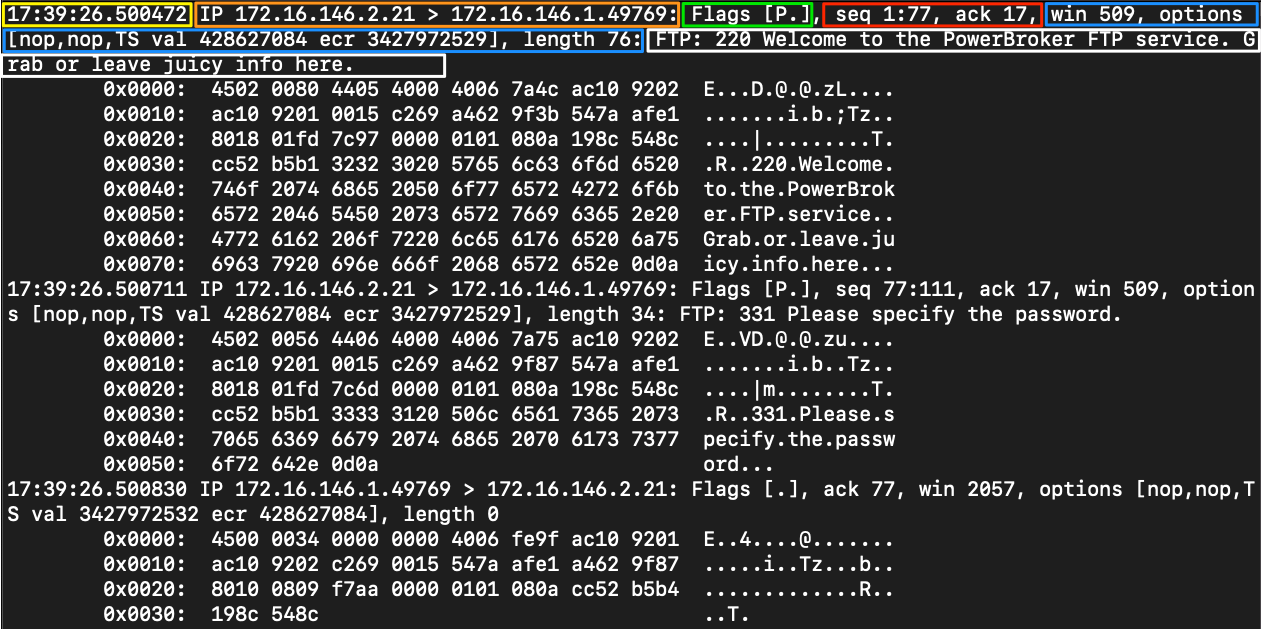
\includegraphics[width=\linewidth]{tools/all/images/tcpdump-out.png}
  \caption{TCPDump output}
  \label{fig:tcpdump-output}
\end{figure}

\begin{tabularx}{\linewidth}{|l|X|}
    \hline
Filter &	Result \\
    \hline
Timestamp &	Yellow The timestamp field (configurable).\\
    \hline
Protocol &	Orange This section will tell us what the upper-layer header is
(here IP).\\
    \hline
Source \& Destination IP.Port &	Orange show the source and destination of the
packet along with the port number used to connect. Format: \verb+IP.port == 172.16.146.2.21+ \\
    \hline
Flags &	Green This portion shows any flags utilized. \\
    \hline
Sequence and Acknowledgement Numbers &	Red shows the sequence and
acknowledgment numbers used to track the TCP segment. \\
    \hline
Protocol Options &	Blue show any negotiated TCP values established between the
client and server, such as window size, selective acknowledgments, window scale
factors, and more.\\
    \hline
Notes / Next Header &	White Misc notes the dissector found will be present
here. As the traffic we are looking at is encapsulated, we may see more header
information for different protocols. In our example, we can see the TCPDump
dissector recognizes FTP traffic within the encapsulation to display it for
us.\\
    \hline
\end{tabularx}


\subsection*{TCPDump Filters}

When utilizing filters, we can apply them directly to the capture or apply them
when reading a capture file. 

see~\ref{network:bpf}

\begin{tabularx}{\linewidth}{|l|X|}
    \hline
Filter &	Result \\
    \hline
host &	host will filter visible traffic to show anything involving the
designated host. Bi-directional\\
    \hline
src / dest &	src and dest are modifiers. We can use them to designate a
source or destination host or port. \\
    \hline
net &	net will show us any traffic sourcing from or destined to the network
designated. It uses / notation. \\
    \hline
proto &	will filter for a specific protocol type. (ether, TCP, UDP, and ICMP as
examples) \\
    \hline
port &	port is bi-directional. It will show any traffic with the specified
port as the source or destination.\\ 
    \hline
portrange &	portrange allows us to specify a range of ports. (0-1024)\\
    \hline
less / greater "< >" &	less and greater can be used to look for a packet or
protocol option of a specific size.\\
    \hline
and / \&\& &	and \&\& can be used to concatenate two different filters
together. for example, src host AND port.\\
    \hline
or &	or allows for a match on either of two conditions. It does not have to
meet both. It can be tricky.\\
    \hline
not &	not is a modifier saying anything but x. For example, not UDP.\\
    \hline
\end{tabularx}

\begin{verbatim}
# Host Filter
### Syntax: host [IP]
sudo tcpdump -i eth0 host 172.16.146.2

# Source/Destination Filter
### Syntax: src/dst [host|net|port] [IP|Network Range|Port]
sudo tcpdump -i eth0 src host 172.16.146.2


sudo tcpdump -i eth0 tcp src port 80
sudo tcpdump -i eth0 dest net 172.16.146.0/24

# Protocol Filter
### Syntax: [tcp/udp/icmp]
sudo tcpdump -i eth0 udp

# Protocol Number Filter
### Syntax: proto [protocol number]
sudo tcpdump -i eth0 proto 17

# Port Filter
### Syntax: port [port number]
sudo tcpdump -i eth0 tcp port 443

# Port Range Filter
### Syntax: port [port number]
sudo tcpdump -i eth0 tcp port 443

# Less/Greater Filter
### Syntax: less/greater [size in bytes]
sudo tcpdump -i eth0 less 64

# AND Filter
### Syntax: and [requirement]
sudo tcpdump -i eth0 host 192.168.0.1 and port 23

# OR Filter
### Syntax: or/|| [requirement]
sudo tcpdump -r sus.pcap icmp or host 172.16.146.1

# NOT Filter
### Syntax: not/! [requirement]
sudo tcpdump -r sus.pcap not icmp

# Looking for TCP Protocol Flags
sudo tcpdump -i eth0 'tcp[13] & 2 != 0'

# Hunting For a SYN Flag
sudo tcpdump -i eth0 'tcp[13] &2 != 0'

\end{verbatim}
